\documentclass{article}
\usepackage{cleveref}
\usepackage{listings}
\usepackage[margin=1in]{geometry}
\usepackage{graphicx}
\graphicspath{{images/}}

\author{Collin Walther \and Phi Lam}
\title{Installation Guide for the SCU Course Equivalency System}

\begin{document}
\maketitle

\section{Introduction}
\par The following installation guide gives instructions on how to set up the
SCU course equivalency system. It makes a few assumptions:
\begin{itemize}
\item The system must be set up on a student account on the Engineering Computing
Center (ECC) computers.
Installation on an arbitrary system is possible, but is not included in the scope
of this document.
\item You must have the 10 necessary PHP source files
(AddFacultyUser.php, AddNewEquivalency.php, AttemptFacultyLogin.php,
EquivalenciesTable.php, HelperFunctions.php, Logout.php, ModifyEquivalency.php,
RemoveEquivalency.php, SoftwareEngineeringProject.php, and ViewEquivalency.php)
required for full operation of the system.
\item You must have the MySQL table definitions, included in
TableDefinitions.sql.
\end{itemize}
Failure to satisfy the above conditions may make installation of the system
impossible.

\section{Database Setup}
\par The SCU course equivalency system uses MySQL database server to store
information about users and course equivalencies. If you do not yet have a MySQL
database server available for use, then follow the steps at
http://wiki.helpme.engr.scu.edu/index.php/MySQL-5 to set up MySQL server on the
ECC computers for yourself.

\par Once you have set up MySQL server, you must create the tables necessary for
this system.  There are two tables you must create: one for users, and one for
equivalencies.  To do this, follow these steps:
\begin{enumerate}
\item Go to https://dagobah.engr.scu.edu/.  It should look like the image in
\cref{fig:dagobah}
\item Click on the ``MySQL Web Interface (phpMyAdmin)'' link.
\item Enter your SCU Unix username/password when prompted. This is the same
username/password that you use to log on to the ECC linux computers.
\item You will be sent to the phpMyAdmin login page. See \cref{fig:phpmyadminlogin}.
Enter your MySQL
username/password (see http://wiki.helpme.engr.scu.edu/index.php/MySQL-5 for
the default username/password, if you have not yet changed yours).
\item You will now be taken to the phpMyAdmin console. See \cref{fig:phpmyadmin}.
Click on the link on the left side of the screen that says sdb\_\textless YOUR
USERNAME\textgreater .
This is the database in which you will create your tables.
\item Click on the ``SQL'' tab at the top of the page. See \cref{fig:dbview}.
\item Copy and paste the entire contents of TableDefinitions.sql into the text
area available on the page. See \cref{fig:sql}.  Click the ``Go'' button on the
right side of the screen.  This creates the tables in your database.  Refresh
the page and examine sdb\_\textless YOUR USERNAME\textgreater  to make sure that
the tables were
created successfully.
\end{enumerate}
\par After completing these steps, the database backend of this system has been
successfully set up.

\section{Installing Bootstrap}
\par This system uses the Bootstrap framework to style the user interface.
Follow these steps to download and install the Bootstrap framework.
\begin{enumerate}
\item Download Bootstrap 3.3 by clicking on the "Download Bootstrap" button at
\newline http://getbootstrap.com/docs/3.3/getting-started/.
\item The downloaded .zip archive, when unpacked, contains 3 directories: css,
js, and fonts. Copy the following 3 files from these directories into your student webpage directory, located on
the ECC computers in the directory /webpages/\textless YOUR USERNAME\textgreater :
\begin{enumerate}
\item css/bootstrap.css
\item css/bootstrap-theme.css
\item js/bootstrap.min.js
\end{enumerate}
\end{enumerate}
\par After following these steps, Bootstrap has been installed on your ECC
student webpage.

\section{Installing PHP Source Files}
\par The next step of the installation process involves installing the source
files on the ECC computers so that they will be served to visitors by the ECC
web server.  To do this, follow the following steps:
\begin{enumerate}
\item Change the source files so that they properly link to your database.
There are 7 source files (AddFacultyUser.php, AddNewEquivalency.php,
AttemptFacultyLogin.php, EquivalenciesTable.php, ModifyEquivalency.php,
RemoveEquivalency.php, and ViewEquivalency.php) that each contain the following 4
lines of code:
\begin{lstlisting}
$db_host = "dbserver.engr.scu.edu";
$db_user = "cwalther";
$db_pass = "a password";
$db_name = "sdb_cwalther";
\end{lstlisting}
In each of the 7 files, change these 4 lines to the following:
\begin{lstlisting}
$db_host = "dbserver.engr.scu.edu";
$db_user = "<YOUR USERNAME>";
$db_pass = "<YOUR MYSQL PASSWORD>";
$db_name = "sdb_<YOUR USERNAME>";
\end{lstlisting}
where \textless YOUR USERNAME\textgreater  is your username and \textless YOUR
MYSQL PASSWORD\textgreater  is your
password for logging into MySQL/phpMyAdmin.
\item Ensure that php-cgi is set up on your account to properly prevent your
database credentials and backend logic from being stolen.  To do so, follow the
steps at \newline http://wiki.helpme.engr.scu.edu/index.php/Webpage\#PHP-CGI.
\item Copy the 10 source files
(AddFacultyUser.php, AddNewEquivalency.php, AttemptFacultyLogin.php,
EquivalenciesTable.php, HelperFunctions.php, Logout.php, ModifyEquivalency.php,
RemoveEquivalency.php, SoftwareEngineeringProject.php, and ViewEquivalency.php)
into /webpages/\textless YOUR USERNAME\textgreater  on an ECC computer.
\item In the command line, navigate to /webpages/\textless YOUR USERNAME\textgreater
and run the
following commands to ensure that your source files are private:
\begin{lstlisting}
chmod 700 AddFacultyUser.php
chmod 700 AddNewEquivalency.php
chmod 700 AttemptFacultyLogin.php
chmod 700 EquivalenciesTable.php
chmod 700 HelperFunctions.php
chmod 700 Logout.php
chmod 700 ModifyEquivalency.php
chmod 700 RemoveEquivalency.php
chmod 700 SoftwareEngineeringProject.php
chmod 700 ViewEquivalency.php
\end{lstlisting}
\end{enumerate}

\par At this point, the entire system should now be installed. To confirm that
the system works, navigate to students.engr.scu.edu/\textasciitilde \textless
YOUR USERNAME\textgreater /SoftwareEngineeringProject.php and verify that you
arrive at the home page.  You should be able to log in as the administrator
(username is ``admin'', password is ``password''), which will allow you to
create faculty users and equivalencies.

\begin{figure}[h]
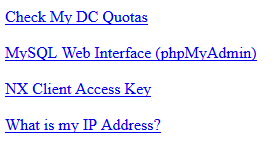
\includegraphics[width=5cm]{dagobah}
\centering
\caption{Dagobah}
\label{fig:dagobah}
\end{figure}

\begin{figure}[h]
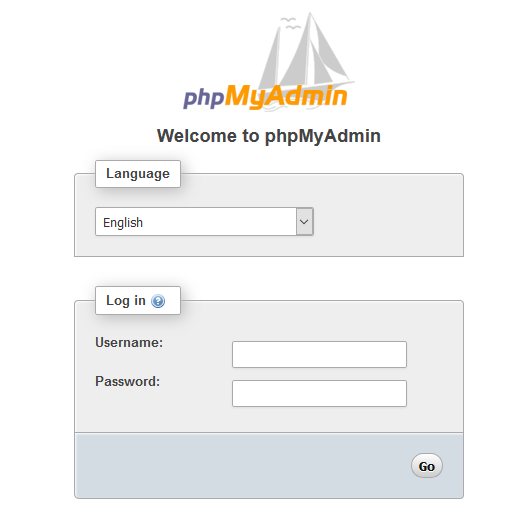
\includegraphics[width=10cm]{phpmyadminlogin}
\centering
\caption{phpMyAdmin login}
\label{fig:phpmyadminlogin}
\end{figure}

\begin{figure}[h]
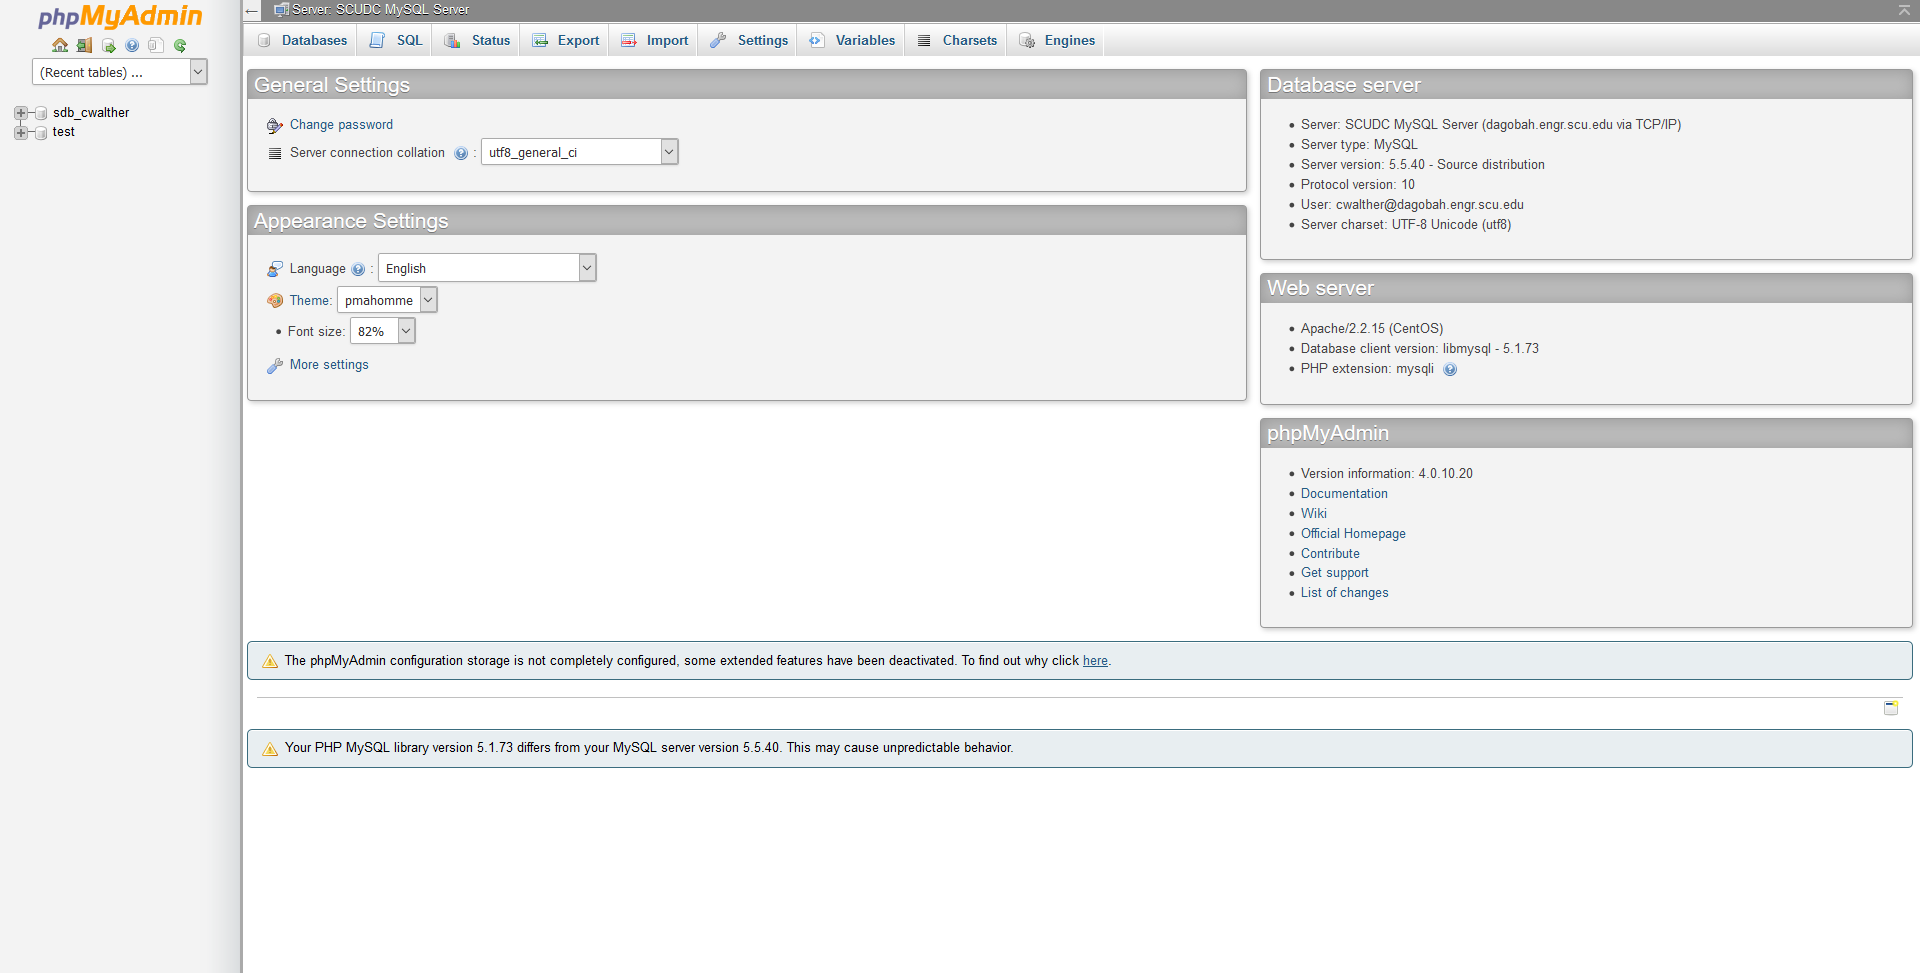
\includegraphics[width=15cm]{phpmyadmin}
\centering
\caption{The phpMyAdmin console}
\label{fig:phpmyadmin}
\end{figure}

\begin{figure}[h]
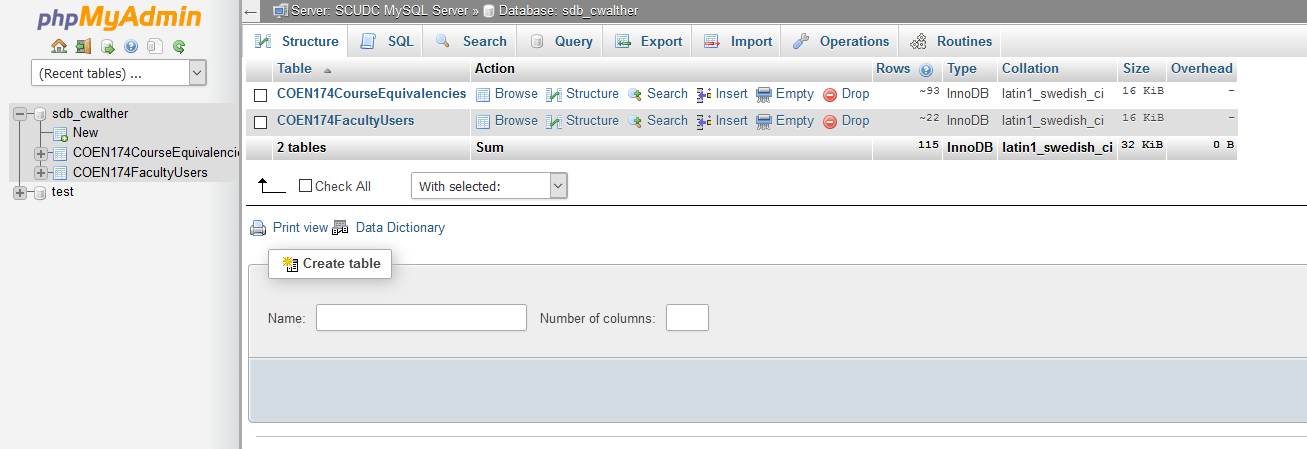
\includegraphics[width=15cm]{dbview}
\centering
\caption{Viewing tables in the database}
\label{fig:dbview}
\end{figure}

\begin{figure}[h]
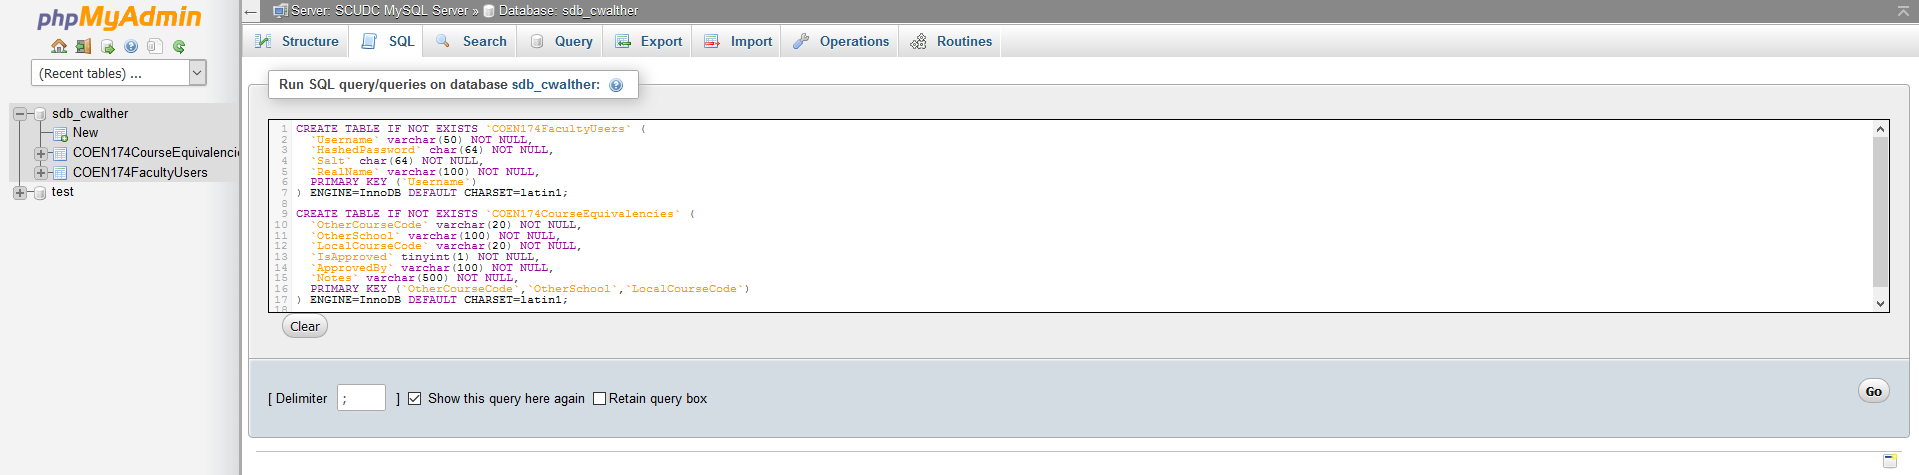
\includegraphics[width=15cm]{sql}
\centering
\caption{Entering SQL through phpMyAdmin}
\label{fig:sql}
\end{figure}

\end{document}
